\documentclass{beamer}
\usetheme{Goettingen}
\usefonttheme[onlymath]{serif}

\usepackage[version=4]{mhchem}
\usepackage{graphicx}
\usepackage{svg}
\usepackage{empheq}
\usepackage[many]{tcolorbox}

\usefonttheme{professionalfonts}
\usepackage{times}
\usepackage{amsmath}
\usepackage{verbatim}

\usepackage{tikz}
\usetikzlibrary{arrows,shapes,positioning,shadows,trees,matrix,math,ipe,calc}
\tikzset{>=stealth}
\newcommand{\tikzmark}[3][]{\tikz[remember picture,baseline] \node [anchor=base,#1,](#2) {#3};}
\def\centerarc[#1](#2)(#3:#4:#5){\draw[#1]($(#2)+({#5*cos(#3)},{#5*sin(#3)})$) arc (#3:#4:#5);}
\tikzstyle{ipe stylesheet} = [
  ipe import,
  even odd rule,
  line join=round,
  line cap=butt,
  ipe pen normal/.style={line width=0.4},
  ipe pen heavier/.style={line width=0.8},
  ipe pen fat/.style={line width=1.2},
  ipe pen ultrafat/.style={line width=2},
  ipe pen normal,
  ipe mark normal/.style={ipe mark scale=3},
  ipe mark large/.style={ipe mark scale=5},
  ipe mark small/.style={ipe mark scale=2},
  ipe mark tiny/.style={ipe mark scale=1.1},
  ipe mark normal,
  /pgf/arrow keys/.cd,
  ipe arrow normal/.style={scale=7},
  ipe arrow large/.style={scale=10},
  ipe arrow small/.style={scale=5},
  ipe arrow tiny/.style={scale=3},
  ipe arrow normal,
  /tikz/.cd,
  ipe arrows, % update arrows
  <->/.tip = ipe normal,
  ipe dash normal/.style={dash pattern=},
  ipe dash dashed/.style={dash pattern=on 4bp off 4bp},
  ipe dash dotted/.style={dash pattern=on 1bp off 3bp},
  ipe dash dash dotted/.style={dash pattern=on 4bp off 2bp on 1bp off 2bp},
  ipe dash dash dot dotted/.style={dash pattern=on 4bp off 2bp on 1bp off 2bp on 1bp off 2bp},
  ipe dash normal,
  ipe node/.append style={font=\normalsize},
  ipe stretch normal/.style={ipe node stretch=1},
  ipe stretch normal,
  ipe opacity 10/.style={opacity=0.1},
  ipe opacity 30/.style={opacity=0.3},
  ipe opacity 50/.style={opacity=0.5},
  ipe opacity 75/.style={opacity=0.75},
  ipe opacity opaque/.style={opacity=1},
  ipe opacity opaque,
]

\definecolor{red}{rgb}{1,0,0}
\definecolor{green}{rgb}{0,1,0}
\definecolor{blue}{rgb}{0,0,1}
\definecolor{yellow}{rgb}{1,1,0}
\definecolor{orange}{rgb}{1,0.647,0}
\definecolor{gold}{rgb}{1,0.843,0}
\definecolor{purple}{rgb}{0.627,0.125,0.941}
\definecolor{gray}{rgb}{0.745,0.745,0.745}
\definecolor{brown}{rgb}{0.647,0.165,0.165}
\definecolor{navy}{rgb}{0,0,0.502}
\definecolor{pink}{rgb}{1,0.753,0.796}
\definecolor{seagreen}{rgb}{0.18,0.545,0.341}
\definecolor{turquoise}{rgb}{0.251,0.878,0.816}
\definecolor{violet}{rgb}{0.933,0.51,0.933}
\definecolor{darkblue}{rgb}{0,0,0.545}
\definecolor{darkcyan}{rgb}{0,0.545,0.545}
\definecolor{darkgray}{rgb}{0.663,0.663,0.663}
\definecolor{darkgreen}{rgb}{0,0.392,0}
\definecolor{darkmagenta}{rgb}{0.545,0,0.545}
\definecolor{darkorange}{rgb}{1,0.549,0}
\definecolor{darkred}{rgb}{0.545,0,0}
\definecolor{lightblue}{rgb}{0.678,0.847,0.902}
\definecolor{lightcyan}{rgb}{0.878,1,1}
\definecolor{lightgray}{rgb}{0.827,0.827,0.827}
\definecolor{lightgreen}{rgb}{0.565,0.933,0.565}
\definecolor{lightyellow}{rgb}{1,1,0.878}
\definecolor{black}{rgb}{0,0,0}
\definecolor{white}{rgb}{1,1,1}
\tcbset{highlight math style={enhanced, colframe=blue!20!black, colback=white, arc=4pt, boxrule=0.5pt}}

\title[Molecular Hydrophobicity Potential]
{%
    Implementing Molecular Hydrophobicity Potential Measurment for the Analysis of Dynamic Biomolecular Interactions
}
\date{\today}
\author[Pelg Bar Sapir]
{
    Peleg Bar Sapir\inst{1} \and \\
    Under supervision of Prof. Maria Andrea Mroginski\inst{2}
}
\institute[Freie Universit\"{a}t Berlin, Techniche Universit\"{a} Berlin]
{
    \inst{1}%
        Freie Universit\"{a}t Berlin
    \and
    \vskip-2mm
    \inst{2}%
        Techniche Universit\"{a}t Berlin
}

\begin{document}
\tikzstyle{every picture}+=[remember picture]
\everymath{\displaystyle}

\begin{frame}
    \titlepage
\end{frame}

\begin{frame}{Outline}
    \tableofcontents
\end{frame}

\section{Introduction}
\subsection{Hydrophobicity and log P}

\section{Molecular Hydrophobicity Potential}
\subsection{Potential}
\subsubsection{General form}

\begin{frame}{The MHP Formula}

    \centering
    \includesvg[scale=0.1]{mhp_visual1}

    \begin{equation*}
        \text{MHP}\left(\mathbf{x'}\right)=
        \tikz[baseline]{
            \node[anchor=base] (sum)
            {$\sum_{i=1}^{k}\limits$};
        }\left[ 
        \tikz[baseline]{
            \node[anchor=base] (force)
            {$f_i$};
        } \cdot
        \tikz[baseline]{
            \node[anchor=base] (distance)
            {$D\left(\mathbf{x}-\mathbf{x'}_i\right)$};
        }\right]
    \end{equation*}

    \begin{tikzpicture}[overlay, remember picture,node distance=1.5cm]
        \uncover<2->{\node[fill=blue!20, xshift=1.2cm, yshift=0.5cm] (sumdescr) [below left=of sum]{Summing over all atoms};}
        \uncover<2->{\draw[->,thick] (sumdescr) to [in=-90,out=90] (sum);}
        \uncover<2->{\node[fill=blue!20] at (sum) {$\sum_{i=1}^{k}\limits$};}
                        
        \uncover<3->{\node[fill=red!20, yshift=-0.2cm] (forcedescr) [below = of force]{Force constants};}
        \uncover<3->{\draw[->,thick] (forcedescr) to [in=-90,out=90] (force);}
        \uncover<3->{\node[fill=red!20] at (force) {$f_i$};}

        \uncover<4->{\node[fill=green!20, xshift=-2.0cm,yshift=0.5cm] (distancedescr) [below right = of distance]{Distance function};}
		\uncover<4->{\draw[->,thick] (distancedescr) to [in=-90,out=90] (distance.south);}
        \uncover<4->{\node[fill=green!20] at (distance) {$D\left(\mathbf{x}-\mathbf{x'}_i\right)$};}
	\end{tikzpicture}
\end{frame}

\subsubsection{Force constants}
\begin{frame}{Force constants}
    \centering
    \begin{tabular}{l l r}
        Type & Description & $f_i$ value \\
        \hline
            & \underline{C in:} &         \\
        3   & $\ce{CHR_3}$      & -0.6681 \\
        15  & $\ce{=CH_2}$      & -0.7866 \\
        36  & $\ce{R-CH-X}$     & -0.2405 \\
            & & \\
            & \underline{H attached to}:                      &         \\
        45  & $\ce{C_{sp^{3}}}$, no X attached to next carbon &  0.7341 \\
        46  & $\ce{C_{sp^{3}}, C_{sp^{2}}}$                   &  0.6301 \\
        50  & Heteroatom                                      & -0.1036 \\
        52  & $\ce{C_{sp^{3}}}$, 1 X attached to next carbon  &  0.6666 \\
            & & \\
            & \underline{O in}: &         \\
        56  & Alcohol           & -0.3567 \\
        58  & Ketone            & -0.0233 \\
        62  & \ce{O-}           & -0.7941 \\
        \hline
    \end{tabular}
    ~\\
    \tiny{Source: Arup K. Ghose et al, J. Phys. Chem. A 1998, 102, 3762-3772}
\end{frame}

\subsubsection{Distance function}
\begin{frame}{Distance function}
    \centering
    \begin{minipage}[t]{0.48\linewidth}
        \centering
        Audry form
        \begin{empheq}[box=\tcbhighmath]{align*}
            D\left(x\right)=\frac{1}{1+x}
        \end{empheq}
    \end{minipage}
    \begin{minipage}[t]{0.48\linewidth}
        \centering
        Exponential decay form
        \begin{empheq}[box=\tcbhighmath]{align*}
            D\left(x\right)=e^{-\alpha x}
        \end{empheq}
    \end{minipage}
    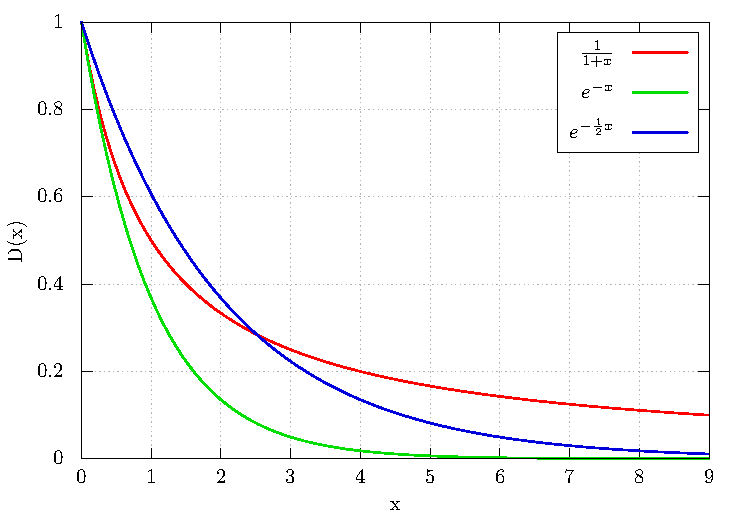
\includegraphics[scale=0.65]{dist_funcs.pdf}    
\end{frame}

\subsection{Surface}
\subsubsection{Solvent accesible surface}
\begin{frame}{Solvent accesible surface}
	\begin{itemize}
		\setlength\itemsep{2em}
		\item The surface around a molecule accesible to solvent molecules \\
		\uncover<2->{
			\item[]
			\begin{tikzpicture}[ipe stylesheet, scale=.75]
				% Scale, distances, coordinates and radii
				\def\scal{0.2}
				\def\dOH{195*\scal}
				\def\dOC{220*\scal}
				\def\RP{120*\scal}
				\coordinate (O) at (230,670);
				\def\RO{152*\scal}
				\def\ROP{\RO+\RP}	
				\coordinate (H) at ($(O)+(\dOH,0)$);
				\def\RH{120*\scal}
				\def\RHP{\RH+\RP}	
				\coordinate (C) at ($(O)-(\dOC,\dOC)$);
				\def\RC{170*\scal}
				\def\RCP{\RC+\RP}

				% Cut radii+probe (should be parameterized...)
				\centerarc[ipe pen heavier, fill=lightblue, dashed](O)(0:365:54);
				\centerarc[ipe pen heavier, fill=lightblue, dashed](H)(-105:105:48);
				\centerarc[ipe pen heavier, fill=lightblue, dashed](C)(98:352:58);

				% Atoms	
				\filldraw[ipe pen fat, fill=red]
				(O) circle[radius=\RO];
				\filldraw[ipe pen fat, fill=white]
				(H) circle[radius=\RH];
				\draw[-, thick] ($(H)+(\RH,0)$) --++(\RP,0);
				\draw[->] ($(H)+(65,20)$) --($(H)+(3*\RH/2,5)$);
				\node[] at ($(H)+(85,25)$) {$R_{\text{probe}}$};
				\filldraw[ipe pen fat, fill=gray]
				(C) circle[radius=\RC];
				\draw[-, thick] (C) --++(-\RC,0);
				\node[] at ($(C)+(-8,8)$) {$R_{\text{vdW}}$};
			\end{tikzpicture}
		}
	\uncover<3->{\item For water molecules usually $r=1.4\left[\text{\AA}\right]$}
	\end{itemize}
\end{frame}

\begin{frame}{How to Create the Solvent Accesible Surface?}
	\centering
	\begin{tikzpicture}[ipe stylesheet, scale=.75]
		% Scale, distances, coordinates and radii
		\def\scal{0.2}
		\def\dOH{195*\scal}
		\def\dOC{220*\scal}
		\def\RP{120*\scal}
		\coordinate (O) at (230,670);
		\def\RO{152*\scal}
		\def\ROP{\RO+\RP}	
		\coordinate (H) at ($(O)+(\dOH,0)$);
		\def\RH{120*\scal}
		\def\RHP{\RH+\RP}	
		\coordinate (C) at ($(O)-(\dOC,\dOC)$);
		\def\RC{170*\scal}
		\def\RCP{\RC+\RP}
	
		% Full radii+probe	
		\uncover<5-8>{\draw[ipe pen heavier]
				      (O) circle[radius=\ROP];}
		\uncover<6-8>{\draw[ipe pen heavier]
				      (H) circle[radius=\RHP];}
		\uncover<7-8>{\draw[ipe pen heavier]
					  (C) circle[radius=\RCP];}
		
		% Cut radii+probe (should be parameterized...)
		\uncover<9- >{\centerarc[ipe pen heavier, fill=white](O)(0:365:54);}
		\uncover<8-8>{\centerarc[ipe pen heavier, red](O)(-58:60:54);}
		\uncover<8-8>{\centerarc[ipe pen heavier, red](O)(165:283:54);}
		\uncover<9- >{\centerarc[ipe pen heavier, fill=white](H)(-105:105:48);}
		\uncover<8-8>{\centerarc[ipe pen heavier, red](H)(105:255:48);}
		\uncover<9- >{\centerarc[ipe pen heavier, fill=white](C)(98:352:58);}
		\uncover<8-8>{\centerarc[ipe pen heavier, red](C)(-8:98:58);}

		% Atoms	
		\uncover<3->{\filldraw[ipe pen fat, fill=red]
		(O) circle[radius=\RO];}
		\uncover<3->{\filldraw[ipe pen fat, fill=white]
		(H) circle[radius=\RH];}
		\uncover<3->{\filldraw[ipe pen fat, fill=gray]
		(C) circle[radius=\RC];}
		
		% Points
		\uncover<1-2>{\coordinate (DV) at (0,10);}
		\uncover<1-2>{\node[] at ($(O)-(DV)$) {O};}
		\uncover<1-2>{\filldraw[black] (O) circle [radius=1];}
		\uncover<1-2>{\node[] at ($(H)-(DV)$) {H};}
		\uncover<1-2>{\filldraw[black] (H) circle [radius=1];}
		\uncover<1-2>{\node[] at ($(C)-(DV)$) {C};}
		\uncover<1-2>{\filldraw[black] (C) circle [radius=1];}
	\end{tikzpicture}
	
	\begin{enumerate}
		\uncover<2->{\item Take all atoms with their vdW-radii}
		\uncover<4->{\item Create spheres around all atoms with $R^{i}=R^{i}_{\text{vdw}}+R_{\text{probe}}$}
		\uncover<8->{\item Delete all points that are "burried" in other extended spheres
			  (i.e. $\Delta\left(p^{i},c^{j}\right)\leq R^{j}+R_{\text{probe}}$)}
		\uncover<9->{\item The remaining surface is the solvent-accesible surface of the molecule}
	\end{enumerate}
\end{frame}

\subsubsection{Evenly distributed points}
\begin{frame}{Evenly distributed points}
    \centering
    How to distribute $N$ points on a surface of a sphere?\\ ~\\ ~\\
    \begin{columns}
        \uncover<1->{
        \begin{column}{0.4\textwidth}
        \centering
	        \includesvg[scale=.17]{sphere_wireframe_coords}\\
        \end{column}
        }
        
        \uncover<3->{
        \begin{column}{0.2\textwidth}
        \centering
	        \includesvg[scale=.17]{arrow_right}
        \end{column}
        \begin{column}{0.4\textwidth}
        \centering
	        \includesvg[scale=.17]{sphere_wireframe_points}
        \end{column}
    }
    \end{columns}
    \begin{columns}
        \begin{column}{0.4\textwidth}
            \begin{itemize}
                \uncover<2->{\item[] $\varphi_{i}=i\cdot\frac{2\pi}{N}$}
                \uncover<2->{\item[] $\theta_{j}=j\cdot\frac{\pi}{N}$}
            \end{itemize}
        \end{column}
        \begin{column}{0.2\textwidth}
        \end{column}
        \begin{column}{0.4\textwidth}
            \begin{itemize}
                \uncover<4->{\item Points are not evenly distributed}
                \uncover<5->{\item Several points overlap at poles}
            \end{itemize}
        \end{column}
    \end{columns}
\end{frame}

\begin{frame}{Evenly distributed points}
    \centering
    Solution: \alert{Vogel's method}\\
    \begin{columns}
        \begin{column}{0.5\textwidth}
            \uncover<1->{In 2 dimensions:}
            \begin{itemize}
                \uncover<2->{\item Distances: $r_{i}=\sqrt{\frac{i}{N}}$}
                \uncover<2->{\item Angle: $\theta_{i}=\varphi i$
                			 \item[] ($\varphi$ is the golden ratio!)}
            \end{itemize}
        \end{column}
        \begin{column}{0.5\textwidth}
			\centering
			\uncover<3->{\includesvg[scale=0.35]{vogels}}
        \end{column}
    \end{columns}
    ~\\ ~\\
    \begin{columns}
        \begin{column}{0.5\textwidth}
            \uncover<4->{In 3 dimensions (cylindrical coordinates):}
            \begin{itemize}
                \uncover<5->{\item Distances: $z_{i}=\left(1-\frac{1}{N}\right)\left(1-\frac{2i}{N-1}\right)$}
                \uncover<5->{\item Angles: $\theta_{i}=\varphi i,\ \rho_{i}=\sqrt{1-z_{i}^{2}}$}
            \end{itemize}
        \end{column}
        \begin{column}{0.5\textwidth}
			\centering
			\uncover<6->{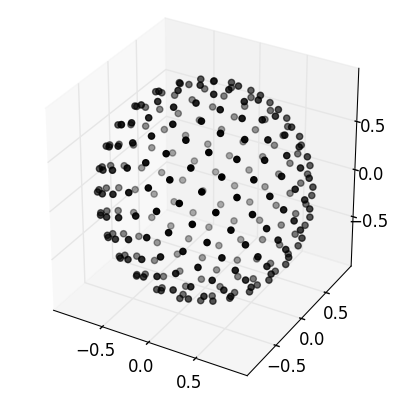
\includegraphics[scale=.4]{3d_vogels.png}\\
                         \tiny{Image source: Marmakoide's Blog}
            }
        \end{column}
    \end{columns}
\end{frame}

\subsubsection{Integration}
\begin{frame}{Integration}
\end{frame}
\end{document}
